%\subsubsection{Illustrative example}
%\label{sec:illustrative example}
\begin{exmp}
\label{ex:toyproblem}
We control the following linear system
\begin{equation}
\label{eq:PointMass}
x_{k+1} = x_k + u_k
\end{equation}
to satisfy the specification
\[\formula = \always_{[0,20]} \neg (x \in \text{Unsafe}) \land \eventually_{[0,20]} (x \in \text{Terminal})\]
with the sets $\text{Unsafe}=[-1,1]^2$ and $\text{Terminal}=[2,2.5]^2$. 
The state space is $X=[-2.5,2.5]^2$, $U=[-0.5,0.5]^2$.
Unless otherwise indicated, we use $\gamma=0$ in Eq. \ref{eq:general_ctrl} to focus on satisfaction in this illustrative example. 
Experiments were run on a quad-core Intel i5 3.2GHz processor with 24GB RAM, running MATLAB 2016b.
%, $\delta=1$, and we optimize for two different values of $\gamma$, $0.1$ and $0.001$. 
%The initial point of the trajectory is $x_0=[-2,-2]'$. 
%Here, $hrz(\formula) = 21$.

\textbf{Results}.
%Fig.~\ref{fig:toy control} shows the sets, initial trajectory (which is unsafe and has a robustness of $-1$), and two trajectories obtained by solving $P_{\srob}$ for two different values of $\gamma$ (with $\delta=0$). Both trajectories satisfy the specification $\formula$. Intuitively, the trajectories in Fig.\ref{fig:toy control} make sense, as for a higher value of $\gamma=0.1$ we get a shorter trajectory, which is closer to unsafe set, hence satisfies $\formula$ less robustly ($\rob_{\formula}=0.65$) and for a smaller value of $\gamma=0.001$ we get a longer trajectory with a higher robustness ($\rob_{\formula}=1.21$).
Fig. \ref{fig:toy control} shows the trajectories of length $N=20$ obtained by SOP and BluSTL in modes (B) and (R), starting from the same initial point $x_0=[-2,-2]'$.
Both BluSTL (B) and SOP (B) produce satisfying trajectories. 
The trajectory from SOP (R) ends in the middle of the terminal set, resulting in a higher robustness than mode (B), as expected. 
In mode (R), BluSTL could not finish a single instance of robustness maximization within 100 hours on both the above machine and on a more powerful 8 core Intel Xeon machine with 60GB RAM, leading us to believe that the corresponding MILP was not tractable.
 
SOP ($\gamma=0.1,\delta=0$) takes into account a control cost $l(x_k,u_k) = ||x_k||_{2}^2$ that penalizes longer trajectories.
The resulting trajectory is shorter but has a lower robustness than SOP (R, $\gamma = 0$), ($0.236$ vs $0.247$).

For further evaluation, we ran 100 instances of the problem, varying the trajectory's initial state in $[-2.5,-1.5] \times [-2.5,2.5]$. 
We also varied the formula horizon $N$ (and hence the size of the problem) from $20$ to $200$ time steps. 
Table \ref{tbl:time_performance_toy} shows the execution times. 


%The control cost is $l(x_k,u_k) = ||x_k||_{2}^2$, so that longer trajectories incur greater cost. 
%Finally, $hrz(\formula) = 21$.
%\todo[inline]{"last trajectory"? reference the legend..}
%\todo[inline]{either call our method Smooth Operator (SOP) or SOP throughout. i strongly suggest the former, because SOP is as forgettable as they come. but most of all, don't use both as you're doing now.}

\begin{table}[tb]
\small
\begin{center}
\caption{{\small Example \ref{ex:toyproblem}. Runtimes (mean and standard deviation, in seconds) for Smooth Operator (SOP) and BluSTL (BlS) in modes (B) and (R), over 100 runs with random initial states and different formula horizons $N$. BluSTL (R) did not finish (see text).}}
\vspace{-5pt}
\label{tbl:time_performance_toy}
\begin{tabular} {|c|c|c|c|c|}
	\hline
	N & BlS(B) & SOP(B) & SOP(R) & SOP(R) \\ \hline
	20 & $0.96 \pm 0.82$ &  $\mathbf{0.31 \pm 0.13}$  & NA & $3.30 \pm 1.25$ \\ \hline
	30 & $1.37 \pm 1.72$ &  $\mathbf{0.33 \pm 0.25}$  & NA & $5.85 \pm 2.74$\\ \hline
	40 & $3.86 \pm 5.10$ &  $\mathbf{0.60 \pm 0.29}$  & NA & $12.36 \pm 6.04$\\ \hline
	50 & $4.36 \pm 12.97$&  $\mathbf{0.74 \pm 0.30}$ & NA & $30.05 \pm 18.23$\\ \hline
	100& $16.77 \pm 27.84$ & $\mathbf{1.21 \pm 0.25}$ & NA & $69.70 \pm 13.16$ \\ \hline
	200& $53.88 \pm 14.18$& $\mathbf{4.19 \pm 1.18}$ & NA & $126.11 \pm 20.43$ \\ \hline
\end{tabular}	
\end{center}
\end{table}

\textbf{Analysis.}
As seen in table \ref{tbl:time_performance_toy}, SOP is consistently faster than BluSTL for the \textit{boolean} mode, and displays smaller variances in runtimes. 
Note also that the problem solved here is very similar to the one used in \cite{Saha_acc16}, which uses another MILP-based method. 
While the underlying dynamics differ and their numbers are reported on a more power machine, these results suggest that our runtimes compare favourably with those in \cite{Saha_acc16}.

%When in Boolean mode, BluSTL results in trajectories with zero robustness (as seen in fig. \ref{fig:toy control}), while our method results in trajectories with an average robustness of 0.10. 
In Robust mode, across all 100 experiments, SOP results in an average $\rob_{\formula}=0.247$ with a standard deviation less than $0.005$. 
This gets very close to the upper bound on robustness, which is 0.25.
This bound is achieved by a trajectory reaching (in less than $N$ time steps) the center of the Terminal set while always staying more than 0.25 distant from Unsafe. 
%Also with this additional knowledge of the global optima upper bound, the SOP method in \textit{robust} mode can be made a lot faster by specifying an exit condition based on a upper threshold of $\srob_{\formula}$ attained at any iteration of the SOP method. While for brevity we do not include results with this additional stopping criteria, it was observed that for an upper bound value of $\srob_{\formula}=0.24$, an average speed up of about $4$-times was observed for $N=20$ and $2$-times for $N=200$ while resulting an average robustness value achieved of $\rob_{\formula} = 0.235$. This shows that with the iterative nature of SQP, we can trade-off performance for improved execution times.
\end{exmp}

\begin{figure}[t]
\centering
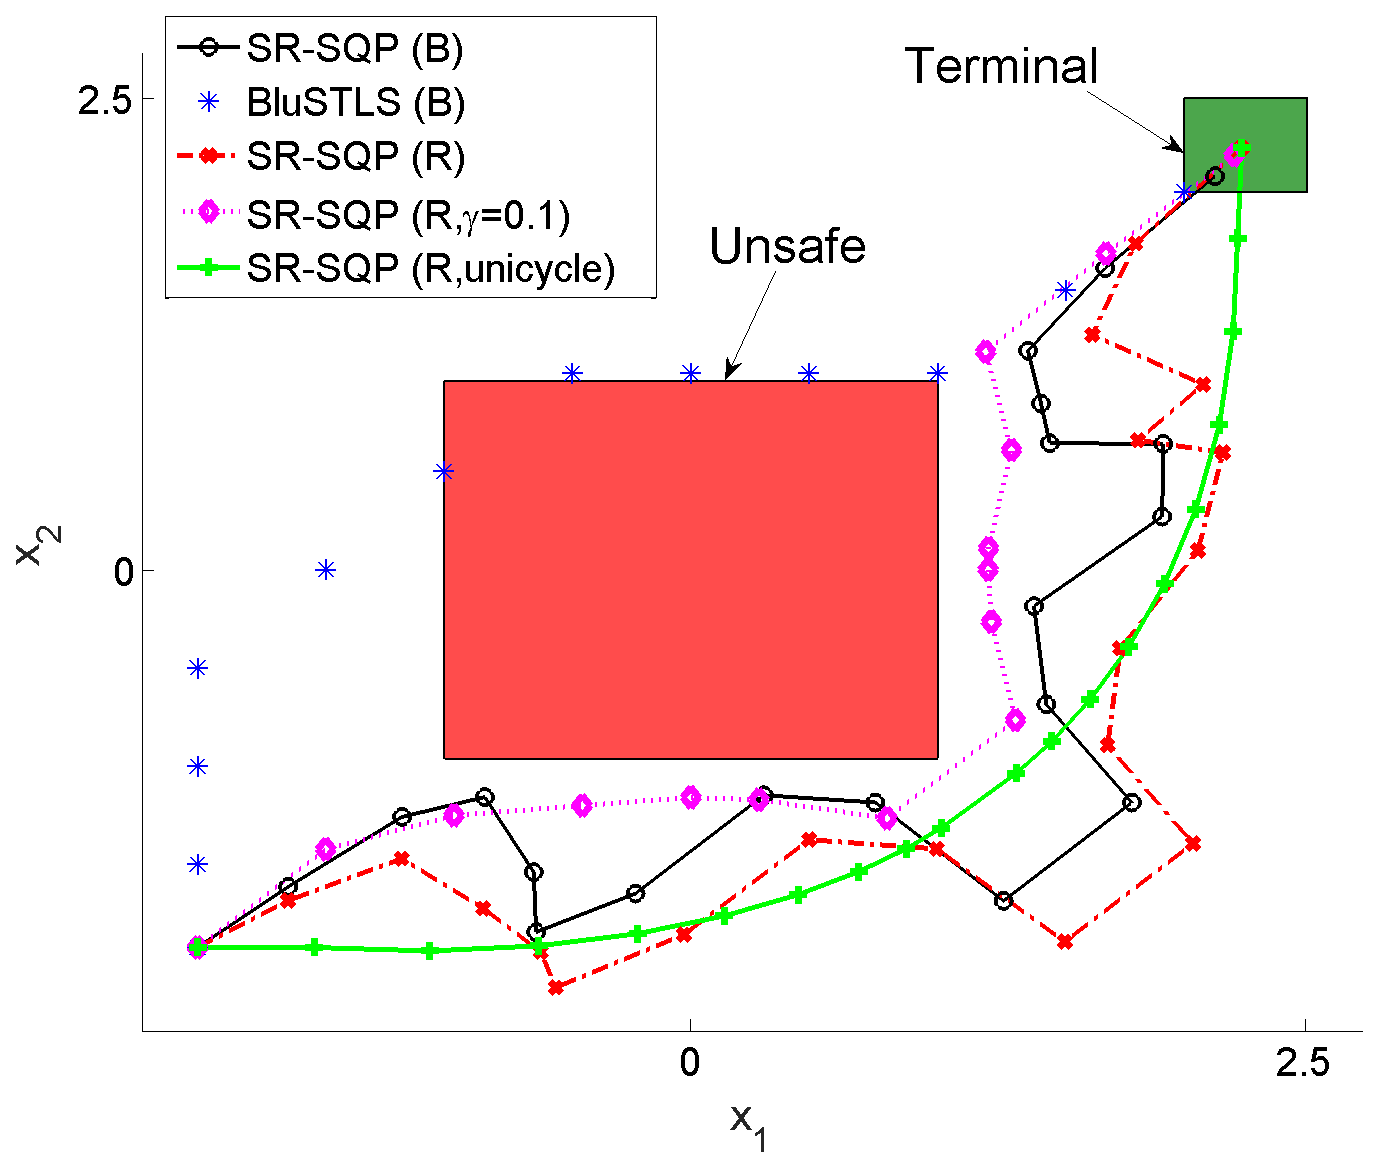
\includegraphics[width=0.49\textwidth]{figures/ToyExUni_scissored.pdf}
\vspace{-20pt}
\caption{{\small The first 4 trajectories are for the linear system \eqref{eq:PointMass}. See Ex. \ref{ex:toyproblem}. The last trajectory, SOP (R, unicycle), is from the non-linear system in Sec. \ref{sec:nl_unicycle}. Colors in online version.}}
\label{fig:toy control}
\vspace{-10pt}
\end{figure}

%\textbf{Optimization solver.}
%We use Sequential Quadratic Programming (SQP) to solve the optimization problem %$P_{\srob}$.
%SQP solves constrained non-linear optimization problems, like $P_{\srob}$, by creating a sequence of quadratic approximations to the problem and solving these approximate problems.
%SQP enjoys various convergence-to-(local)-optima properties, depending on the assumptions we place on the problem. 
%See \cite[Section 2.9]{Polak97_Optim}.
%For example, for SQP to converge to a strict local minimum (a minimum that is strictly smaller than any objective function value in an open neighborhood around it), it suffices that 
%1) all constraint functions be twice Lipschitz continuously differentiable. 
%In our case, this includes function $f$ in \eqref{eq:general ctrl obj}, and the problems we solve satisfy this requirement.
%We will need to assume that $f$ is twice Lipschitz continuously differentiable and that its gradient $f_u$ has maximum row rank.
%And, 
%2) at points in the search space that lie on the boundary of the inequality-feasible set (where the inequality constraints are satisfied with equality), there exists a search direction towards the interior of the feasible set that does not violate the equality constraints (the so-called Mangasarian-Fromowitz constraint qualification) \cite[Assumption 2.9.1]{Polak97_Optim}.
%This is also true in our case since our equality constraints come from the dynamics and are always enforced for any $\mathbf{u}$.

%\textbf{Solver initialization}.
%To initialize SQP when solving $P_{\srob}$ (i.e., give it a starting value for $\mathbf{u}$), we can either:

% a) solve an inexpensive feasibility linear program with constraints \eqref{eq:general ctrl dyn}-\eqref{eq:general ctrl U}. By definition, the resulting trajectory simply satisfies the constraints without optimizing the objective.
 
% b) or, generate a random input sequence respecting $u_k \in U$. 
% Such a trajectory will be very fast to generate and feasible w.r.t the dynamics but is unlikely to satisfy the specification on the system. 

%Note, the resulting initial trajectory is free to violate the specification (as it does in every example we study in this paper) and we only enforce that it satisfy the dynamics and state constraints.
